\documentclass[pdf, ]{beamer}
\usepackage[]{hyperref, graphicx, siunitx, lmodern, tikz, booktabs, physics}
\usepackage[mode=buildnew]{standalone}
\usepackage{pdfpc-commands}
\usepackage{intro-commands}
\pgfplotsset{compat=1.16}

\usetheme{Astro}
\graphicspath{ {Images/} }

\sisetup{per-mode=symbol}
\usetikzlibrary{calc, patterns, decorations.markings, decorations.pathmorphing, shapes}

%Preamble
\title{A Tour and Guide to Salem's Night Skies}
\author{Jed Rembold}
\date{August 3, 2019}

\begin{document}
\renewcommand{\theenumi}{\Alph{enumi}}

{
	\setbeamertemplate{footline}{}
	\maketitle
}

\begin{frame}{Overview}
	\begin{itemize}
		\item The Moon
			\begin{itemize}
				\item Tycho
				\item Copernicus
				\item Sea of Tranquility
			\end{itemize}
		\item Planets
			\begin{itemize}
				\item Jupiter and moons
				\item Saturn
				\item Venus and Mars
			\end{itemize}
		\item Deep Sky
			\begin{itemize}
				\item Pleides
				\item Orion Nebula
				\item Andromeda Galaxy
				\item Hercules Cluster
			\end{itemize}
		\item Perseid Meteor Shower
	\end{itemize}
\end{frame}

\section{The Moon}

\begin{frame}{The Moon}
	\begin{itemize}
		\item Where to find:
			\begin{itemize}
				\item Full: highest in sky around midnight
				\item New: highest in sky at noon
				\item Waxing: up in early evening
				\item Waning: up in early morning
			\end{itemize}
		\item Always see basically the same side of the Moon
			\begin{itemize}
				\item Rotates on axis at same rate it rotates around Earth
			\end{itemize}
		\item Near-side has lots of contrast with darker lowlands and brighter highlands
		\item Looking along the \alert{terminator} where light meets dark, will give the greatest sense of depth and contrast from shadows.
	\end{itemize}
\end{frame}

\begin{frame}{Tycho}
	\begin{columns}
		\column{0.4\textwidth}
		\begin{itemize}
			\item Named after Tycho Brahe
			\item Bright crater in Southern hemisphere
			\item Characterized by many long rays emanating outwards
			\item Fairly young by crater standards
		\end{itemize}
		\column{0.6\textwidth}
		\begin{center}
			\begin{tikzpicture}[scale=0.78]
				\node<1-2> {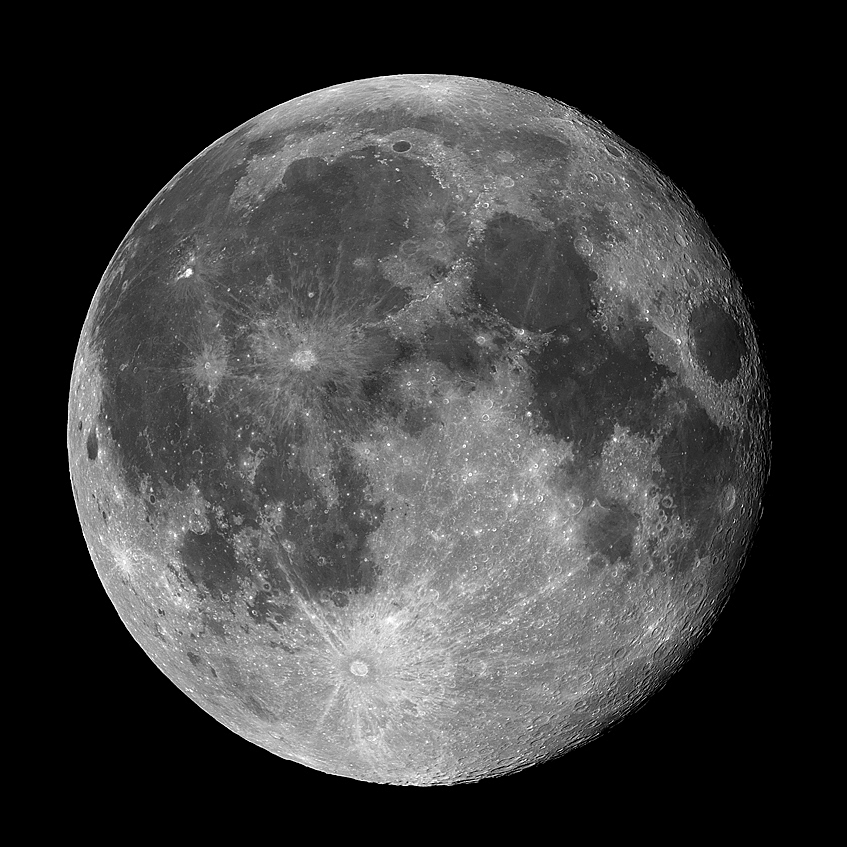
\includegraphics[width=0.8\textwidth]{FullMoon_Barrett.jpg}};
				\draw<2>[very thick, red] (-.5,-1.9) circle (4mm);
				\node<3> {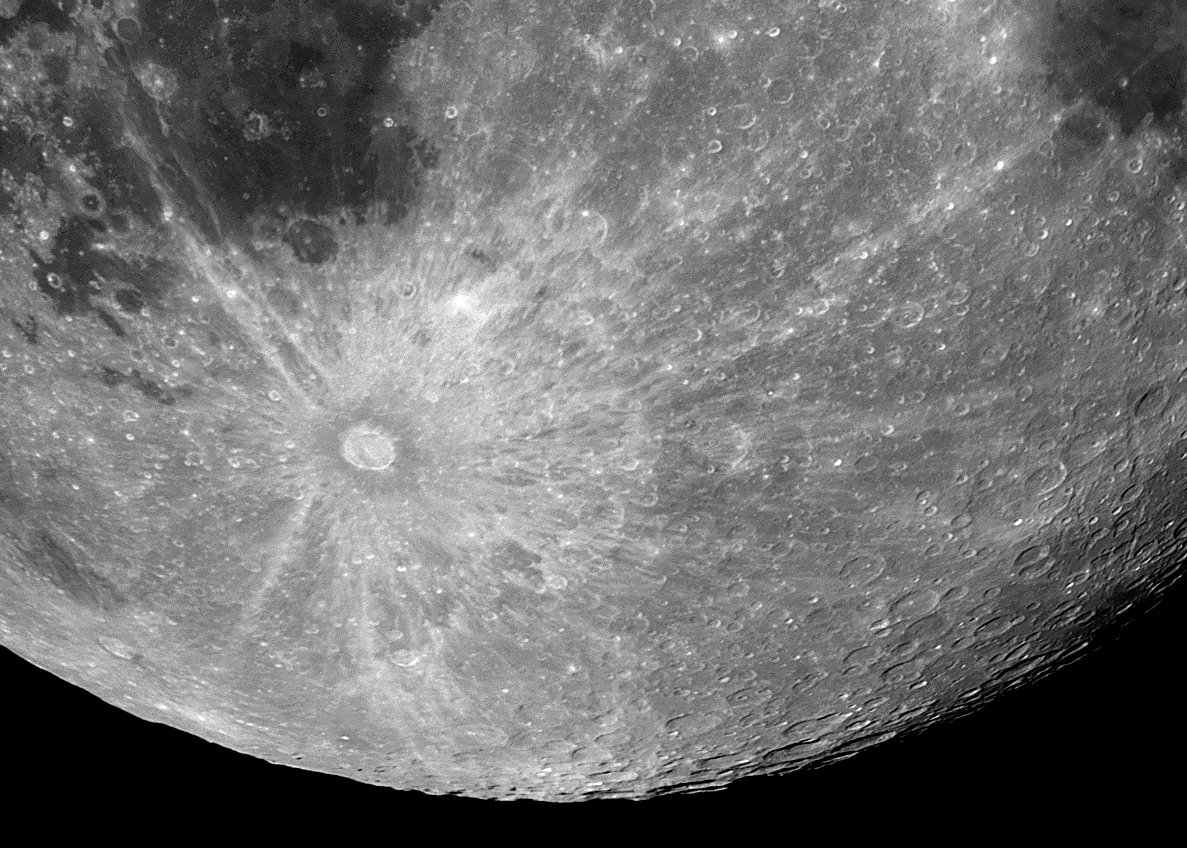
\includegraphics[width=0.9\textwidth]{Tycho_Full_Barrett.jpg}};
			\end{tikzpicture}
		\end{center}
	\end{columns}
\end{frame}

\begin{frame}{Copernicus}
	\begin{columns}
		\column{0.5\textwidth}
		\begin{center}
			\begin{tikzpicture}[scale=0.78]
				\node<1-2> {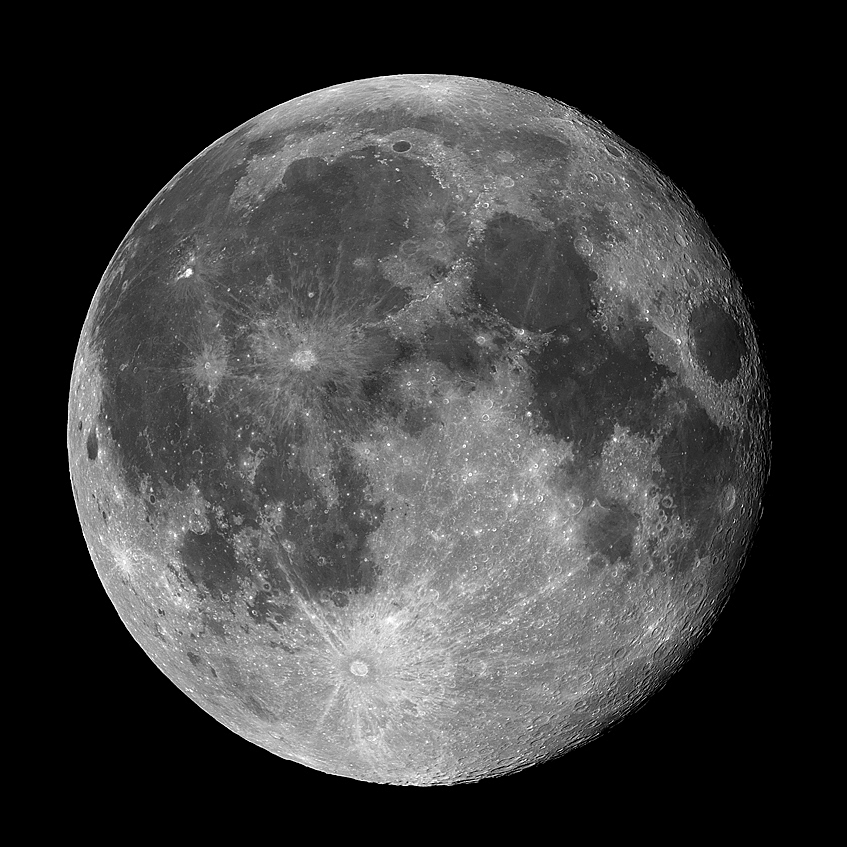
\includegraphics[width=0.9\textwidth]{FullMoon_Barrett.jpg}};
				\draw<2>[very thick, red] (-.9,.5) circle (4mm);
			\end{tikzpicture}
		\end{center}
		
		\column{0.5\textwidth}
		\begin{itemize}
			\item Named after Nicolaus Copernicus
			\item Large crater to West and in center of many darker seas
			\item Also has rays but they are more wandering
		\end{itemize}
		
	\end{columns}
\end{frame}

\begin{frame}{Sea of Tranquility}
	\begin{columns}
		\column{0.5\textwidth}
		\begin{itemize}
			\item Lower of the two seas to the East
			\item Lowlands expose darker rock, giving the distinct shade
			\item Apollo 11 landing was near the Southwest edge
		\end{itemize}
		\column{0.5\textwidth}
		\begin{center}
			\begin{tikzpicture}[scale=0.78]
				\node<1-3> {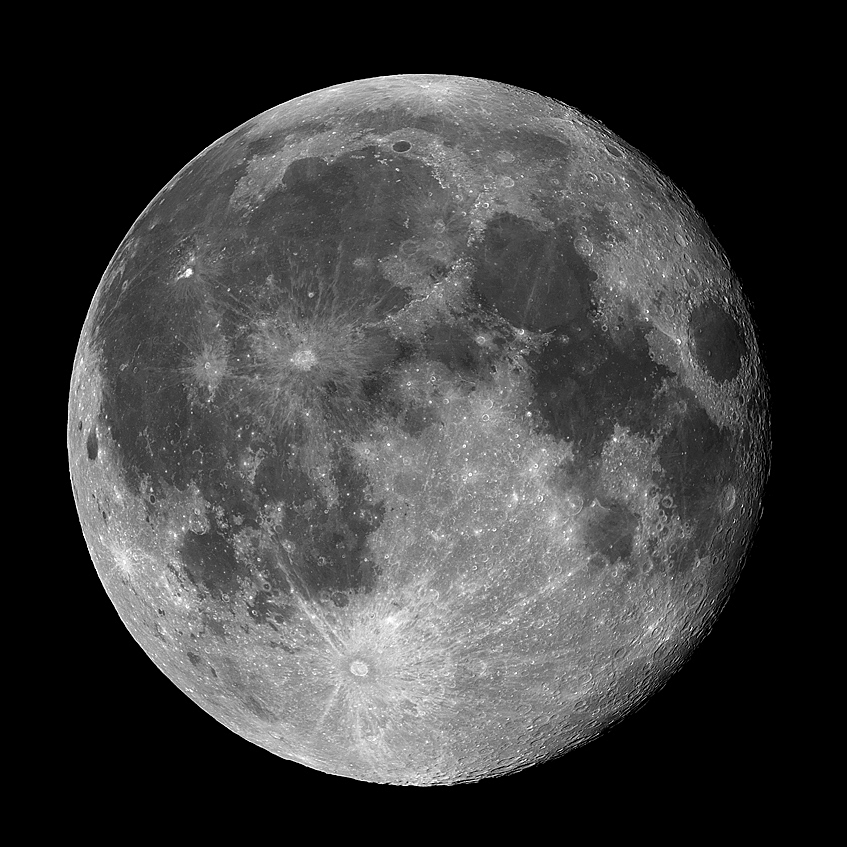
\includegraphics[width=0.9\textwidth]{FullMoon_Barrett.jpg}};
				\draw<2>[very thick, red] (1.2,0.2) circle (8mm);
				\draw<3>[very thick, orange] (1.1,-0.1) circle (2mm);
			\end{tikzpicture}
		\end{center}
	\end{columns}
\end{frame}

\section{The Planets}

\begin{frame}{Jupiter}
	\begin{columns}
		\column{0.55\textwidth}
		\begin{center}
			\begin{tikzpicture}
				\node<1> {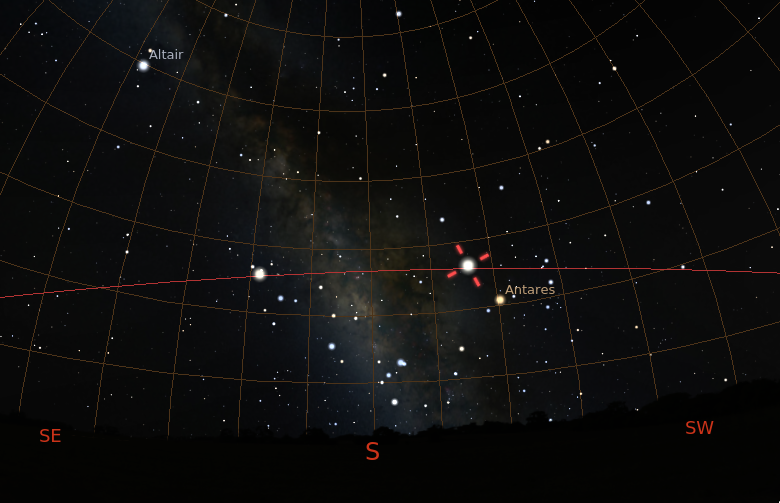
\includegraphics[width=\textwidth]{JupiterPosition.png}};
				\node<2> {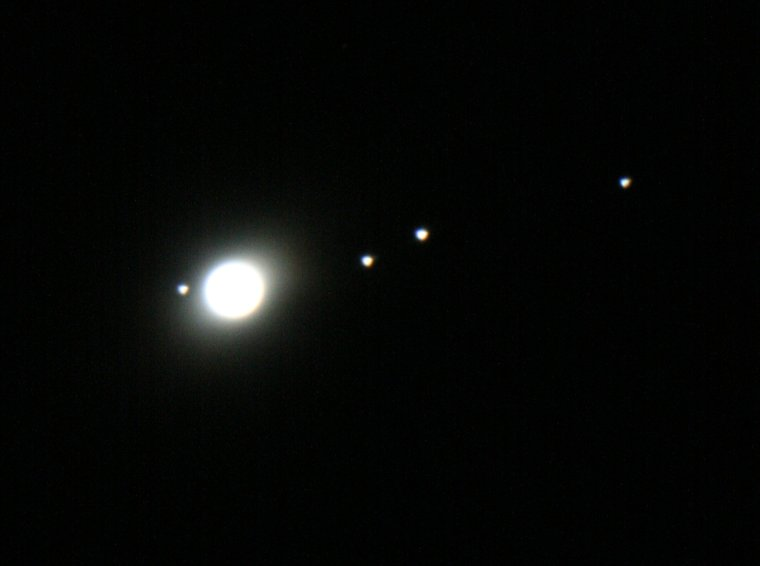
\includegraphics[width=\textwidth]{JupiterMoons.jpg}};
			\end{tikzpicture}
		\end{center}
		
		\column{0.5\textwidth}
		\begin{itemize}
			\item Largest of the planets. Will appear as a very large bright star in the sky.
			\item Look towards the South between 15 and 30 degrees above the horizon.
			\item If you see two really bright stars, Jupiter is the brighter and is the rightmost one at the moment.
			\item 4 moons easily visible with just binoculars
				\begin{itemize}
					\item Io, Europa, Ganymede and Callisto
					\item Sometimes 1 or 2 may be in front or behind the planet
				\end{itemize}
		\end{itemize}
	\end{columns}
\end{frame}

\begin{frame}{Saturn}
	\begin{columns}
		\column{0.5\textwidth}
		\begin{itemize}
			\item Also appears as a bright star in the sky.
			\item Currently near Jupiter but is the more leftmost bright point.
			\item Will just appear oblong in binoculars, really need a \alert{small telescope} to see the rings.
			\item Can sometimes see its largest moon Titan nearby.
		\end{itemize}
		\column{0.5\textwidth}
		\begin{center}
			\begin{tikzpicture}
				\node<1> {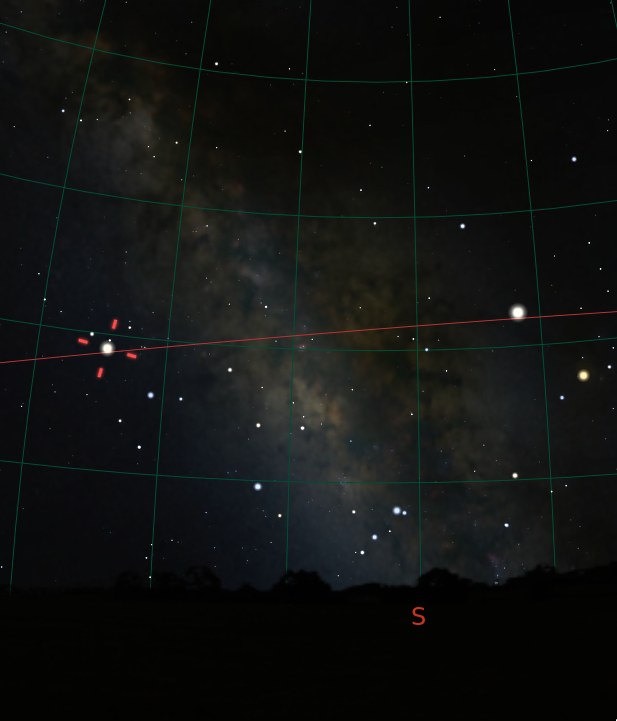
\includegraphics[width=\textwidth]{SaturnPosition.png}};
				\node<2> {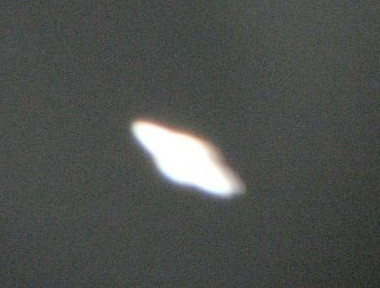
\includegraphics[width=\textwidth]{Saturn-through-binoculars.jpg}};
			\end{tikzpicture}
		\end{center}
		
	\end{columns}
\end{frame}

\begin{frame}{Venus and Mars}
	\begin{columns}
		\column{0.4\textwidth}
		\begin{center}
			\begin{tikzpicture}
				\node<1> {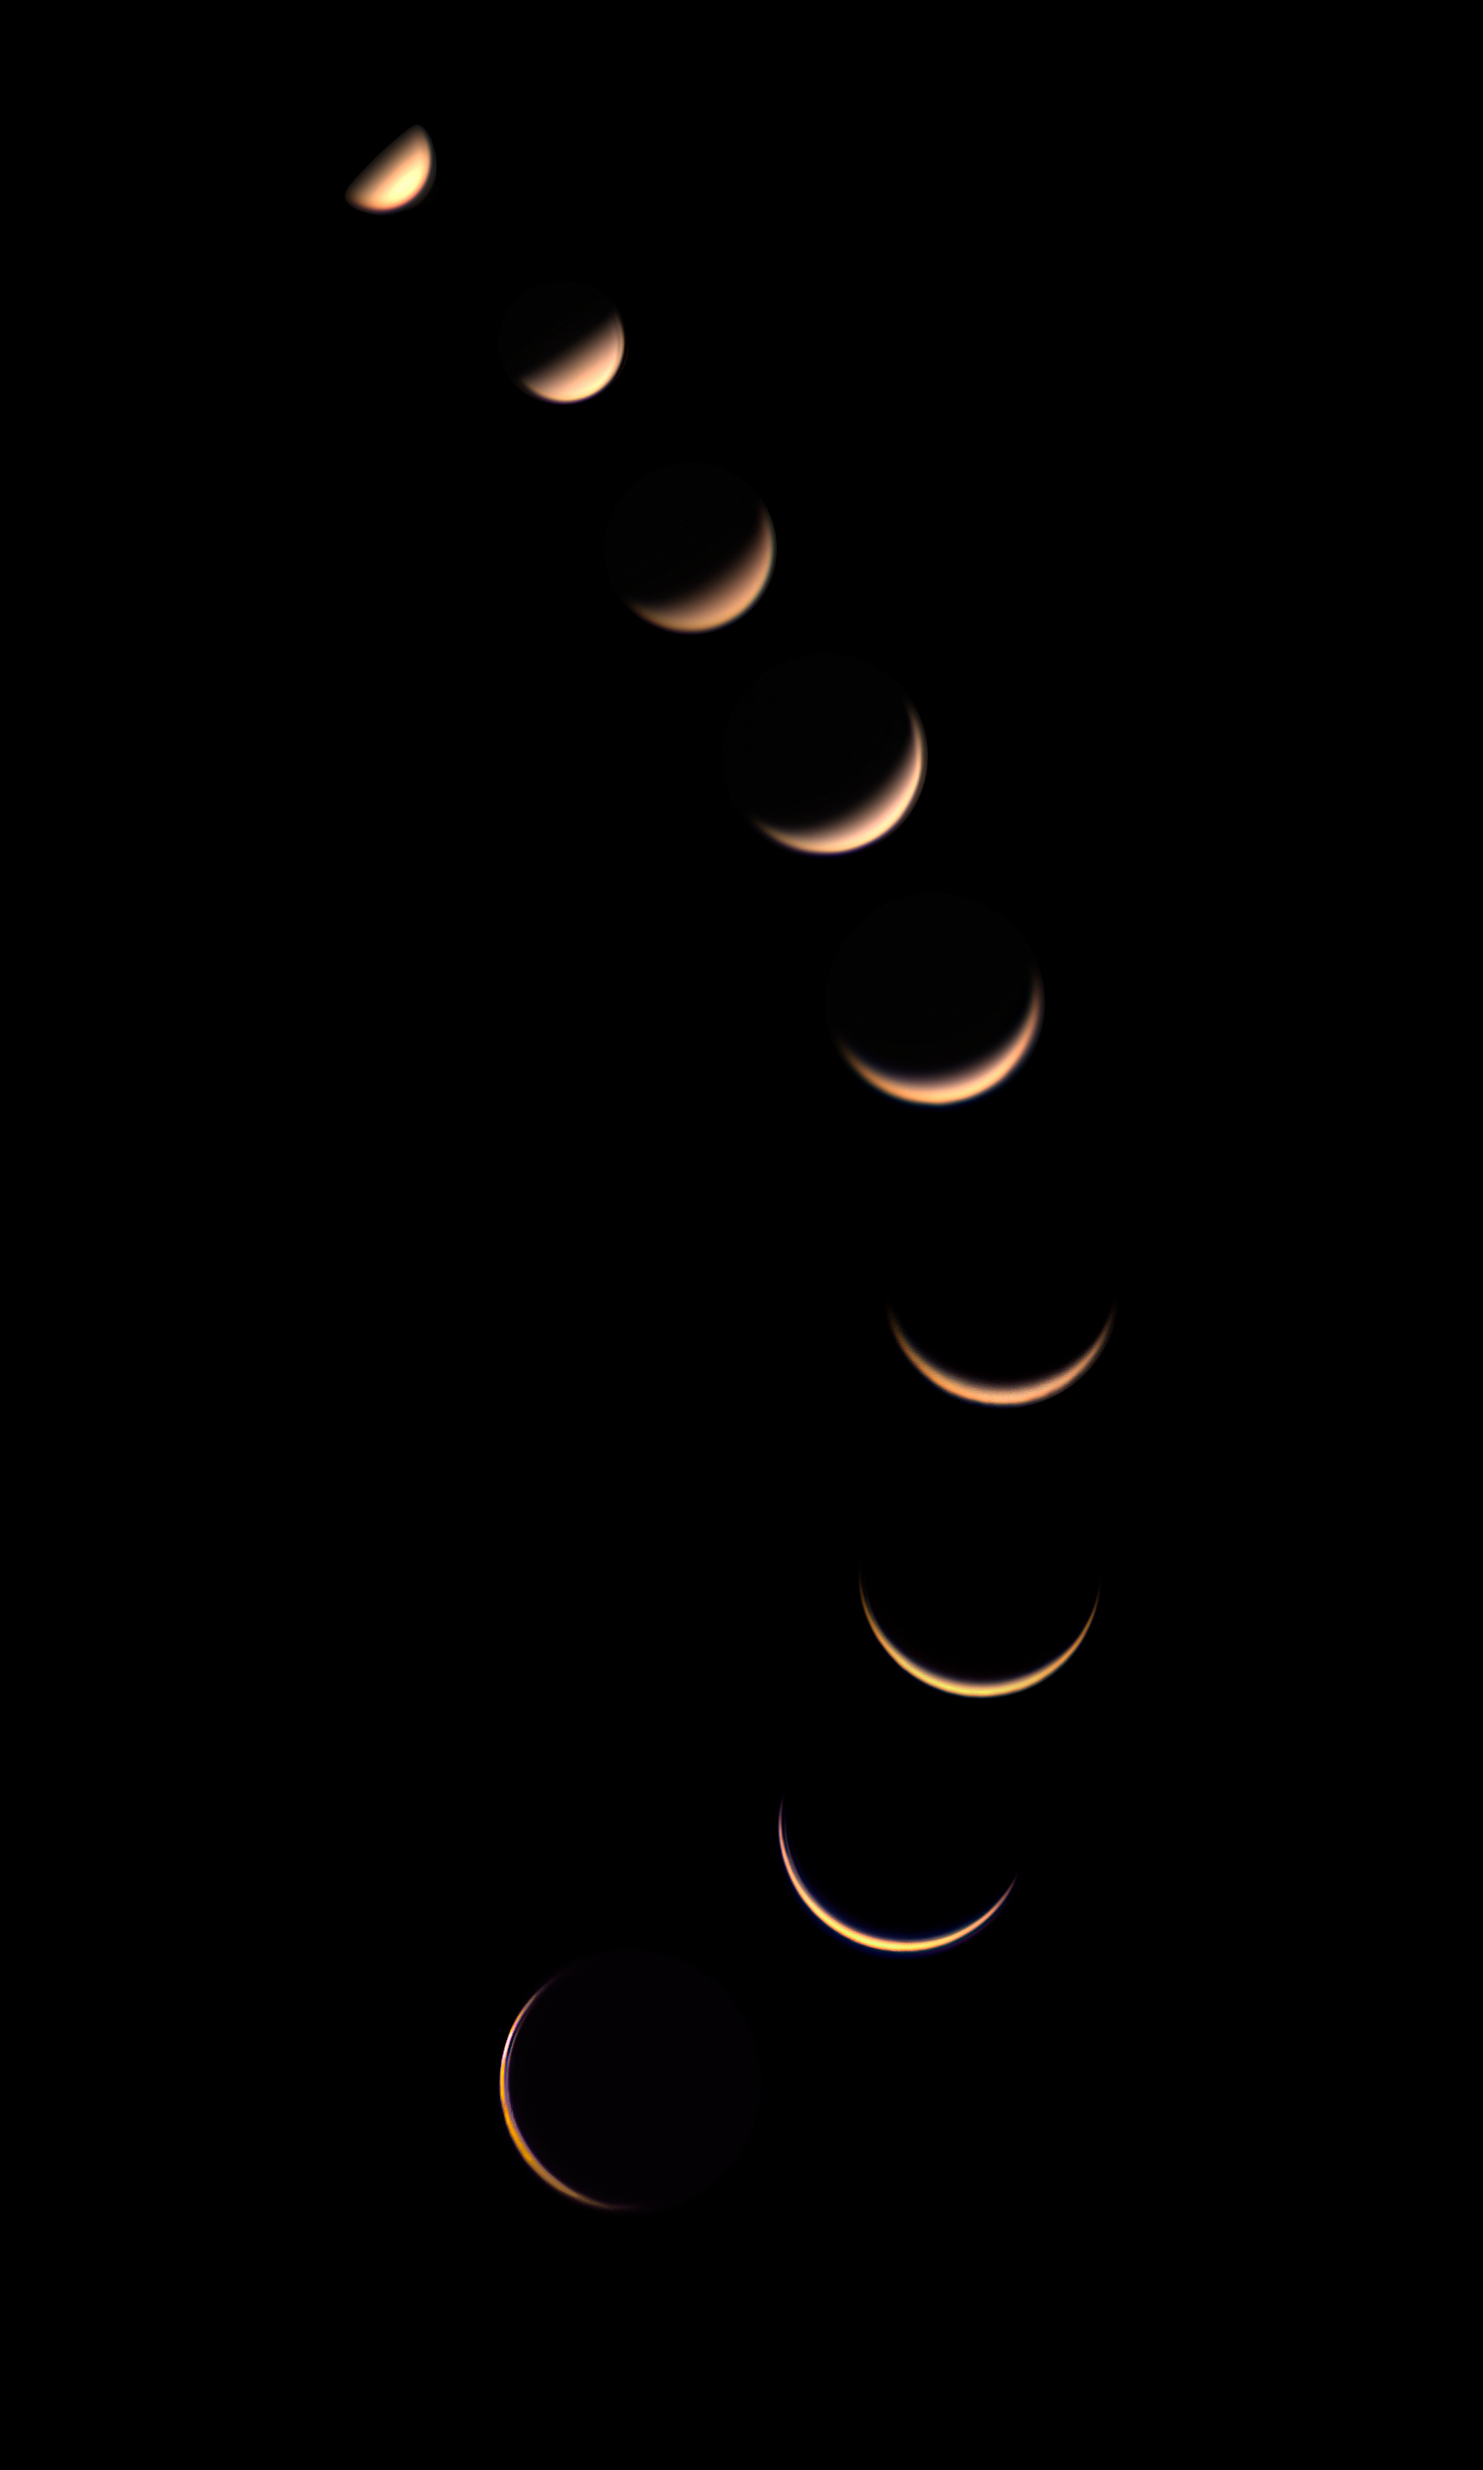
\includegraphics[width=.9\textwidth]{VenusPhases.jpg}};
				\node<2> {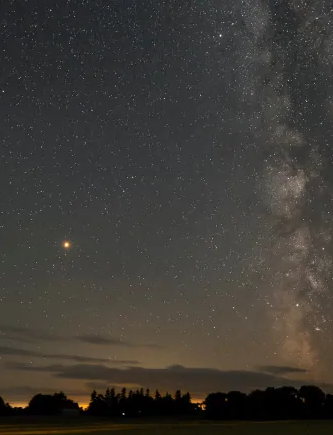
\includegraphics[width=\textwidth]{mars-opposition.png}};
			\end{tikzpicture}
		\end{center}
		\column{0.6\textwidth}
		\begin{itemize}
			\item<1-> Venus
				\begin{itemize}
					\item Brightest planet besides Jupiter
					\item Will always be hanging out near the Sun, so visible only in early evening or morning
						\begin{itemize}
							\item Currently so close to the Sun as to be invisible
						\end{itemize}
					\item Goes through visible phases and size changes
				\end{itemize}
			\item<2-> Mars
				\begin{itemize}
					\item Exhibits a reddish tinge
					\item Lies on the same elciptic, so visible to mostly looking South
					\item With telescope can sometimes make out polar caps
				\end{itemize}
		\end{itemize}
	\end{columns}
\end{frame}

\section{Deep Sky}

\begin{frame}{Andromeda Galaxy}
	\begin{columns}
		\column{0.5\textwidth}
		\begin{itemize}
			\item Our nearest galactic neighbor!
			\item Definitely easier to spot away from light pollution
			\item Follow a trail of constellations to help find it:
				\begin{itemize}
					\item Cassiopeia (the ``W'')
					\item Pegasus (a big square)
					\item Andromeda (two ``legs'' attached to the square)
				\end{itemize}
			\item Will appear an oblong fuzzy blob with naked eyes, much more detail visible with binoculars
		\end{itemize}
		
		\column{0.5\textwidth}
		\begin{center}
			\vspace{-5mm}
			\begin{tikzpicture}[
				star/.style={circle, minimum size=1mm, inner sep=0pt,},
				scale=0.78
				]
				\node {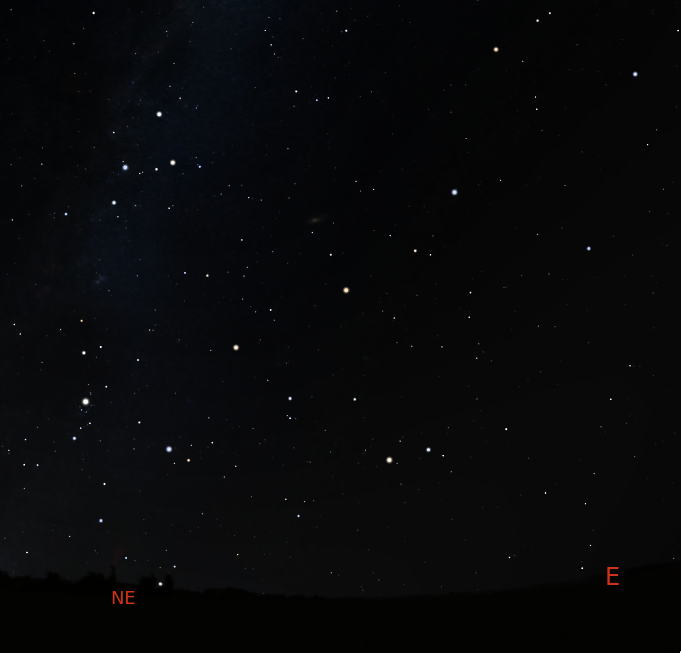
\includegraphics[width=\textwidth]{Cass_n_Peg.png}};
				\node[star] (c1) at (-2.82,1.15) {};
				\node[star] (c2) at ($(c1)+(.5,.12)$) {};
				\node[star] (c3) at ($(c2)+(.11,.37)$) {};
				\node[star] (c4) at ($(c3)+(.48,.06)$) {};
				\node[star] (c5) at ($(c4)+(-.14,.48)$) {};

				\node[star] (p1) at (1.18,1.37) {};
				\node[star] (p2) at ($(p1)+(.43,1.47)$) {};
				\node[star] (p3) at ($(p2)+(1.43,-.26)$) {};
				\node[star] (p4) at ($(p3)+(-.48,-1.78)$) {};

				\node[star] (a1) at ($(p1)+(-.41,-.59)$) {};
				\node[star] (a2) at ($(a1)+(-.71,-.4)$) {};
				\node[star] (a3) at ($(a2)+(-1.14,-.6)$) {};
				\node[star] (a4) at ($(p1)+(-.66,-.44)$) {};
				\node[star] (a5) at ($(a4)+(-.62,-.20)$) {};
				\node[star] (a6) at ($(a5)+(-1.5,-.20)$) {};

				\draw<2->[red, thick] (c1) -- (c2) -- (c3) -- (c4) -- (c5);
				\draw<3->[orange, thick] (p1) -- (p2) -- (p3) -- (p4) -- (p1);
				\draw<4->[cyan,thick] (p1) -- (a1) -- (a2) -- (a3) (p1) -- (a4) -- (a5) -- (a6);
				\draw<5->[green,-latex, thick] (a2) -- ($(a2)!1.9!(a5)$);
			\end{tikzpicture}
		\end{center}
	\end{columns}
\end{frame}

\begin{frame}{Andromeda thru Binoculars}
	\begin{center}
		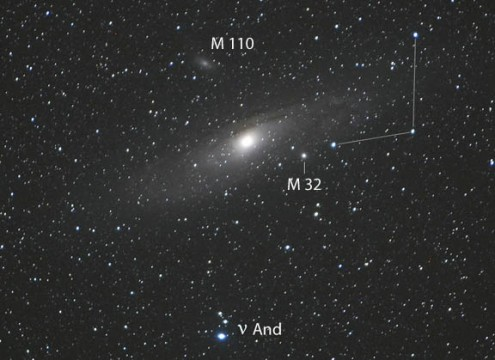
\includegraphics[width=0.8\textwidth]{AndromedaGalaxy.jpg}
	\end{center}
\end{frame}

\begin{frame}{Orion Nebula}
	\begin{columns}
		\column{0.5\textwidth}
		\begin{itemize}
			\item Brightest nebula to look at in the Northern hemisphere
			\item Resides in the ``dagger'' on Orion's belt
			\item Orion currently rises just before the Sun, but will be up earlier and earlier as we move toward winter.
		\end{itemize}
		\column{0.5\textwidth}
		\begin{center}
			\begin{tikzpicture}
				\node<1> {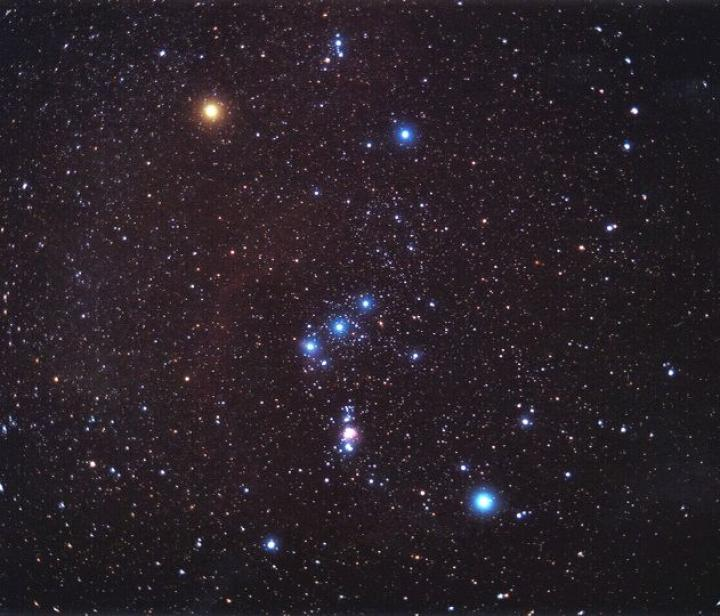
\includegraphics[width=\textwidth]{orion_constellation.jpg}};
				\node<2> {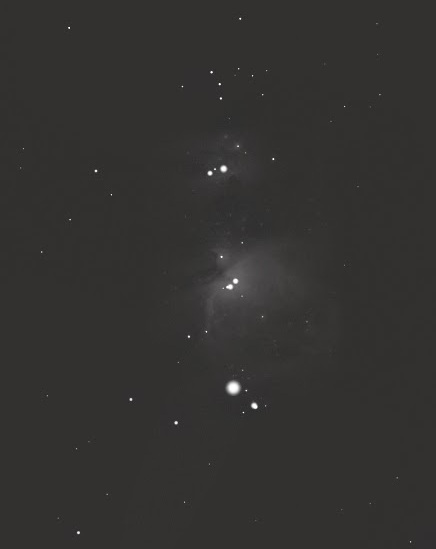
\includegraphics[width=\textwidth]{OrionNebula_Binocs.jpg}};
			\end{tikzpicture}
		\end{center}
	\end{columns}
\end{frame}

\begin{frame}{The Pleides: An Open Star Cluster}
	\begin{columns}
		\column{0.5\textwidth}
		\begin{center}
			\vspace{-8mm}
			\begin{tikzpicture}
				\node<1> {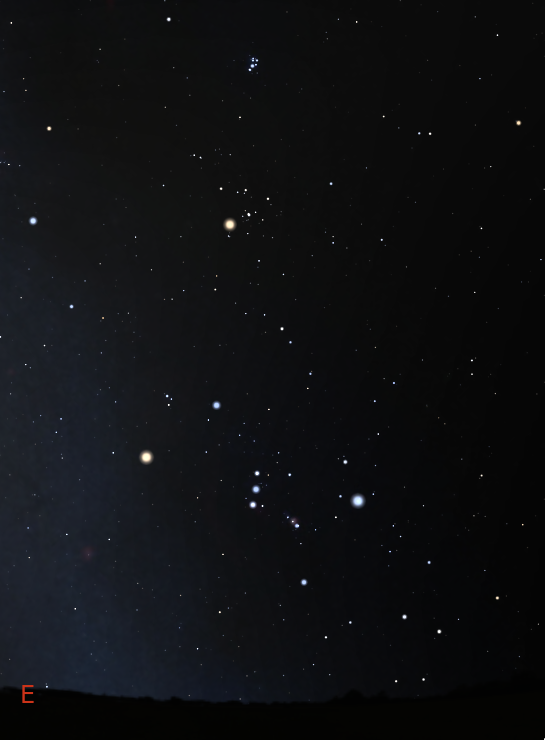
\includegraphics[width=\textwidth]{FindingPleides.png}};
				\node<2> {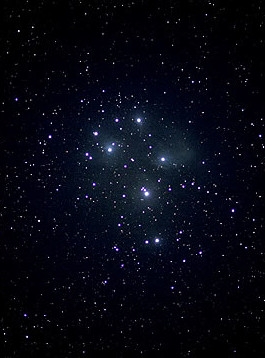
\includegraphics[width=\textwidth]{Pleides.jpg}};
			\end{tikzpicture}
		\end{center}
		\column{0.5\textwidth}
		\begin{itemize}
			\item Located in the constellation Taurus
				\begin{itemize}
					\item Can find by following the line of Orion's belt
					\item Or rapidly scan the sky looking for a blurry spot
				\end{itemize}
			\item Tightly pack bunch of young, bright blue stars
			\item Inspired the Subaru logo
		\end{itemize}
	\end{columns}
\end{frame}



\end{document}

